\chapter{Project scheduling dataset overview}
\label{chap:dataset}

This chapter \changed{presents} the empirical ground this thesis is evaluated on. It
introduces the benchmark instance families used throughout
(Section~\ref{sec:benchmark-datasets}), the structure of an individual
problem instance (Section~\ref{sec:instance-structure}), and the schedule
quality metric and statistical protocol used to compare algorithms
(Section~\ref{sec:eval-metrics}), before Chapter~\ref{chap:approach} turns
to the algorithm itself.

%==============================================================================
\section{Benchmark datasets (PSPLIB, MMLIB)}
\label{sec:benchmark-datasets}
%==============================================================================

Reproducible comparison of scheduling algorithms relies on standardised
benchmark instances with known structure and, where available, published
reference results. This thesis draws on two related families of multi-mode
project-scheduling instances: the Project Scheduling Problem Library
(PSPLIB)~\cite{kolisch1997} and the Multi-Mode Library
(MMLIB)~\cite{vanpeteghem2014}, both distributed in the same plain-text
\texttt{.mm} format described in Section~\ref{sec:instance-structure}.

\subsection{PSPLIB}
\label{subsec:psplib}

PSPLIB~\cite{kolisch1997} is the original and most widely used benchmark
library for the RCPSP and its multi-mode extension. Its multi-mode instance
sets are organised by the number of non-dummy activities $n$ and the number
of modes per activity, and include the well-known j20, j30 and m5 sets
(554, 640 and 558 instances of $n=20$, $n=30$ and $n=16$ activities
respectively, each with 2 renewable and 2 nonrenewable resource types,
following the same resource structure as MMLIB at a smaller scale).
PSPLIB is described here for completeness, as the benchmark family the
wider MRCPSP literature surveyed in Chapter~\ref{chap:overview} most
commonly reports against; this thesis's own comprehensive evaluation
(Chapter~\ref{chap:experiments}) is conducted entirely on MMLIB50 and
MMLIB100 (Section~\ref{subsec:mmlib}), not on PSPLIB, so that every
reported comparison uses one consistent, directly comparable benchmark
family throughout.

\subsection{MMLIB and MMLIB+}
\label{subsec:mmlib}

MMLIB~\cite{vanpeteghem2014} was purpose-built for the MRCPSP and is
substantially larger and more diverse than the PSPLIB multi-mode sets. It
comprises two instance sets:

\begin{itemize}
  \item \textbf{MMLIB50}: 540 instances with $n=50$ activities;
  \item \textbf{MMLIB100}: 540 instances with $n=100$ activities.
\end{itemize}

Both sets share the same resource layout as PSPLIB (2 renewable and 2
nonrenewable resource types, 3 modes per activity) but systematically vary
the instance characteristics described in
Section~\ref{subsec:indicators} (network density, resource availability and
the number of resources actually used by each activity) to produce a wide
and controlled spread of instance difficulty. MMLIB50 and MMLIB100 are the
primary benchmark sets used throughout this thesis: they are the sets on
which the GPHH baseline of Tian et al.~\cite{Tian2024GPHH} was originally
evaluated, and they form the training, validation and test splits used for
the proposed approach in Chapter~\ref{chap:approach} and for the comparative
evaluation in Chapter~\ref{chap:experiments}.

\textbf{MMLIB+} extends this design to 3\,240 instances (648 classes of 5
instances each), split evenly between $n=50$ and $n=100$ activities. Unlike
MMLIB50/100, both the renewable and the nonrenewable resource count vary
between 2 and 4 types per instance, every activity is required to consume
every available resource type (resource factor fixed at 1), and the number
of modes per activity is set to 3, 6 or 9, substantially raising the
dimensionality of the mode-assignment problem and making the nonrenewable
budget a non-trivial constraint rather than a value the baseline can
effectively ignore. This is exactly the setting the
nonrenewable-resource-aware terminals of
Section~\ref{subsec:nr-terminals-definition} are designed for, and a
separate, smaller-scale, instance-matched preliminary check on MMLIB+
(Section~\ref{subsec:nr-eval}) found the same direction of effect as the
main MMLIB50/MMLIB100 evaluation; MMLIB+ is not itself part of this
thesis's comprehensive evaluation.

Table~\ref{tab:datasets} summarises all three families for reference; only
MMLIB50 and MMLIB100 (bold) are used in this thesis's own comprehensive
evaluation (Chapter~\ref{chap:experiments}), PSPLIB and MMLIB+ are included
for context and comparison against the wider literature.

\begin{table}[htbp]
  \centering
  \caption{Multi-mode benchmark instance families referenced in this
  thesis. MMLIB50 and MMLIB100 (bold) are the sets this thesis's
  comprehensive evaluation is conducted on; PSPLIB and MMLIB+ are shown for
  context and are not part of that evaluation.
  $|\mathcal{R}^{\rho}|$ and $|\mathcal{R}^{\nu}|$ denote the number of renewable and
  nonrenewable resource types, respectively; for MMLIB+ these quantities vary
  per instance across the listed values rather than being fixed.}
  \label{tab:datasets}
  \begin{tabular}{l r r r r r}
    \toprule
    \textbf{Dataset} & \textbf{Instances} & \textbf{Activities $n$} & \textbf{Modes} & $|\mathcal{R}^{\rho}|$ & $|\mathcal{R}^{\nu}|$ \\
    \midrule
    PSPLIB j20  & 554   & 20      & 3 & 2 & 2 \\
    PSPLIB j30  & 640   & 30      & 3 & 2 & 2 \\
    PSPLIB m5   & 558   & 16      & 5 & 2 & 2 \\
    \textbf{MMLIB50}     & 540   & 50      & 3 & 2 & 2 \\
    \textbf{MMLIB100}    & 540   & 100     & 3 & 2 & 2 \\
    MMLIB+      & 3\,240 & 50 / 100 & 3 / 6 / 9 & 2 / 4 & 2 / 4 \\
    \bottomrule
  \end{tabular}
\end{table}

%==============================================================================
\section{Data instance structure}
\label{sec:instance-structure}
%==============================================================================

Every instance in PSPLIB and MMLIB is stored as a plain-text file in the
PSPLIB ``multi-mode'' (\texttt{.mm}) format, organised into four blocks: a
header describing the instance size and resource types, a
\emph{precedence relations} block defining the activity-on-node graph of
Section~\ref{subsec:cpm}, a \emph{requests/durations} block giving the
duration and resource requirements of every (activity, mode) pair, and a
\emph{resource availabilities} block giving the capacity of each resource
type. The excerpt below shows part of an MMLIB50 instance file
(\texttt{J50100\_1.mm}, 52 jobs, i.e.\ 50 activities plus a dummy source and
sink); activity~2 illustrates how its three modes trade off duration against
resource consumption (visualised directly in Figure~\ref{fig:mode-tradeoff}).

\begin{samepage}
\begin{code}
jobs (incl. supersource/sink): 52
RESOURCES
  - renewable    : 2 R
  - nonrenewable : 2 N
************************************************
PRECEDENCE RELATIONS:
jobnr.  #modes  #successors  successors
1       1       8             2 3 4 5 6 7 8 11
2       3       6             20 17 16 15 14 13
...
************************************************
REQUESTS/DURATIONS
jobnr. mode  dur  R1  R2  N1  N2
1      1     0    0   0   0   0
2      1     2    0   5   9   9
       2     5    5   0   3   5
       3     6    5   0   2   1
...
************************************************
RESOURCE AVAILABILITIES
       R1  R2  N1   N2
       40  31  289  292
\end{code}
\end{samepage}

\begin{figure}[htbp]
  \centering
  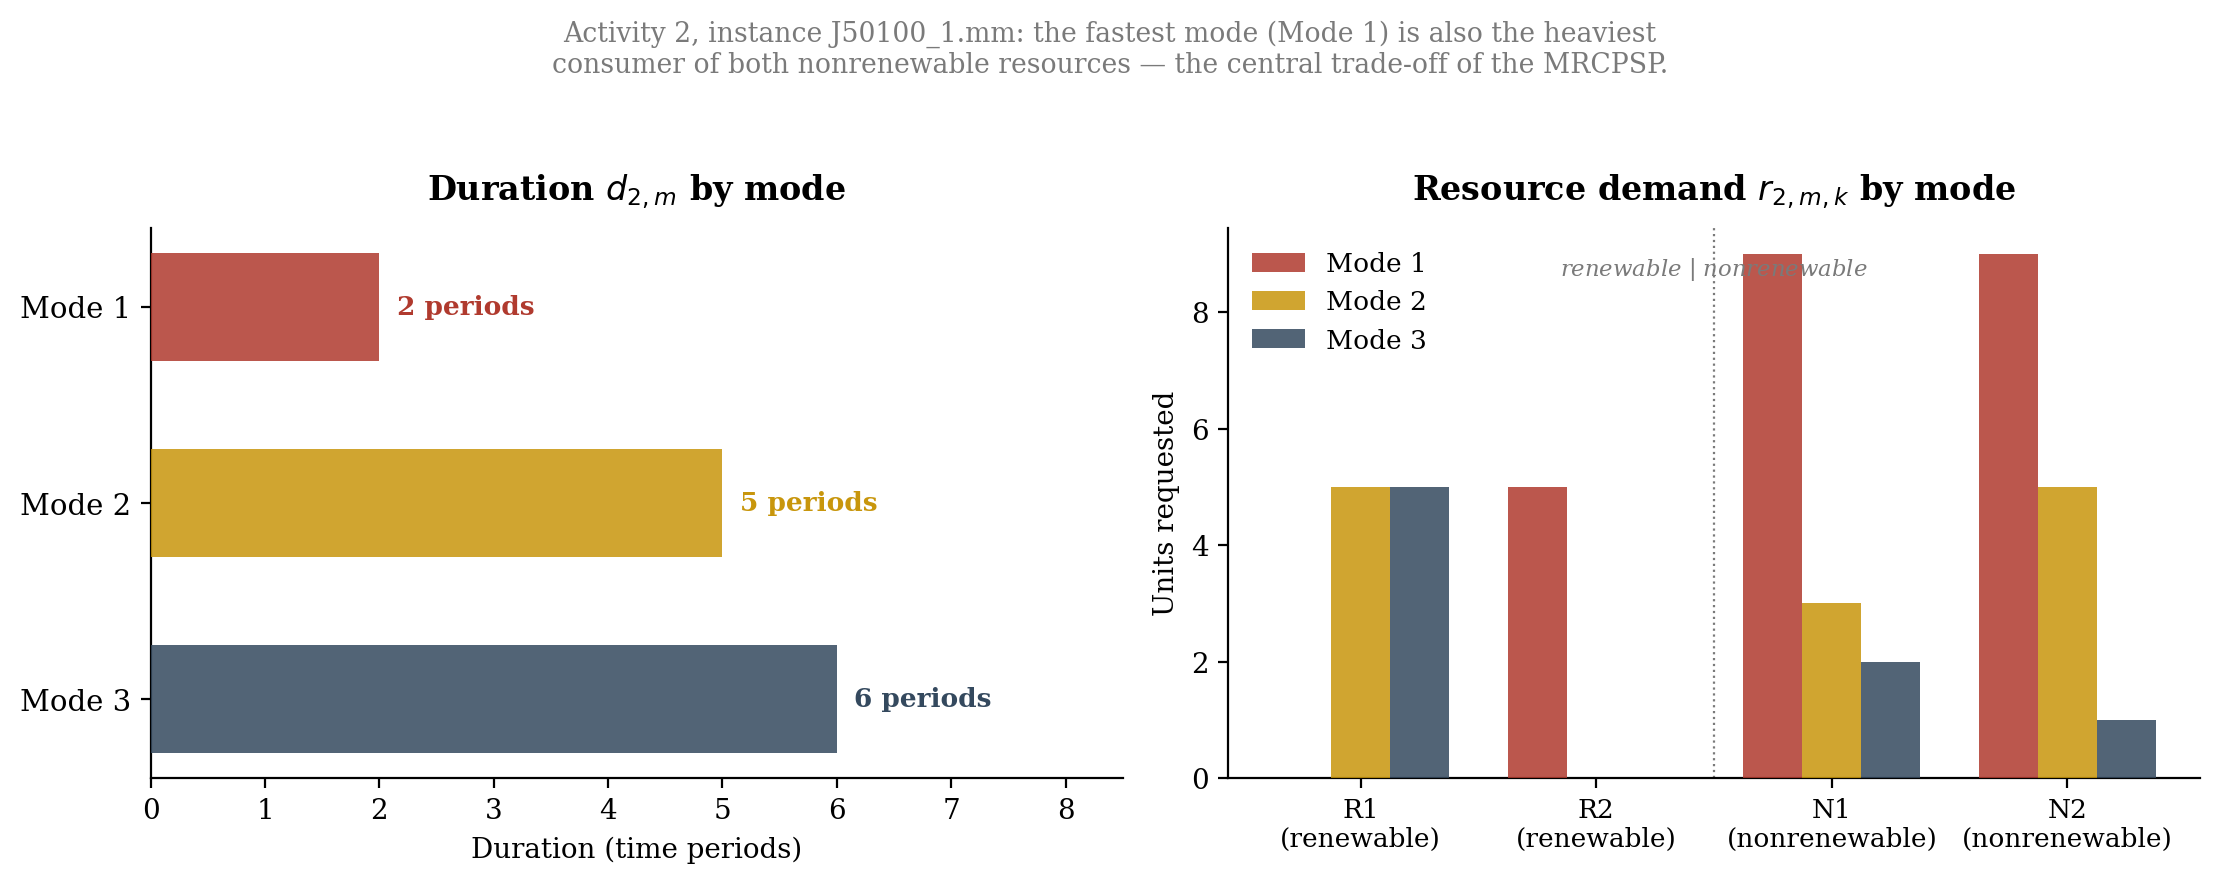
\includegraphics[width=0.95\textwidth]{img/mode-tradeoff.png}
  \caption[Duration vs.\ resource trade-off across modes]{The duration
  vs.\ resource-consumption trade-off across the three modes of activity~2
  in the excerpt above. Left: mode~1 is the fastest. Right: mode~1 is also
  the heaviest consumer of both nonrenewable resources N1 and N2, while
  modes~2 and~3 trade additional duration for a lighter nonrenewable
  footprint: the mode-choice trade-off central to the MRCPSP
  (Section~\ref{subsec:problem-statement}).}
  \label{fig:mode-tradeoff}
\end{figure}

The header fixes the total number of jobs, including the two zero-duration
dummy activities that act as a unique source and sink for the
activity-on-node network of Section~\ref{subsec:cpm}, and the number of
renewable and nonrenewable resource types. The precedence block lists, for
every activity, its number of modes and its immediate successors, which
together define the precedence graph. The requests/durations block then
gives, for every mode $m \in \mathcal{M}_i$ of activity $i$, the duration $d_{im}$ and
the per-period requirement $r_{imk}$ of every resource $k$: choosing a mode
fixes both quantities simultaneously, so a shorter mode (e.g.\ activity~2,
mode~1, duration~2) typically demands more of one resource and less of
another than a longer mode (mode~3, duration~6); this is the mode-choice
trade-off central to the MRCPSP (Section~\ref{subsec:problem-statement}).
Finally, the availabilities block gives the per-period capacity of each
renewable resource and the total project budget of each nonrenewable
resource.

\changedB{When an instance is loaded, the parser produces a model object exposing the
activities, their modes (with per-mode durations and resource requirements),
the precedence relations and the capacities of both resource classes
programmatically; this is the representation queried directly by the GP
terminals and the schedule-generation scheme described in
Chapter~\ref{chap:approach}.}

\subsection{Instance characterisation indicators}
\label{subsec:indicators}

To produce a controlled spread of instance difficulty, MMLIB instances are
generated to target specific values of three pre-existing project- and
resource-characterisation indicators (order strength, resource factor and
resource strength) which Van Peteghem and Vanhoucke adopt when
constructing the dataset~\cite{vanpeteghem2014}.

\textbf{Order strength (OS)} is the density of the precedence graph. Let
$V' = V \setminus \{0, n+1\}$ be the non-dummy activities and let $\mathcal{P}
\subseteq V' \times V'$ be the transitive closure of the precedence edge set
$E$ (Section~\ref{subsec:rcpsp-model}) restricted to $V'$, i.e. $\mathcal{P}$
contains every directly \emph{and} transitively implied precedence relation
between non-dummy activities. OS is then $|\mathcal{P}|$ divided by the
maximum possible number of relations among $n$ activities,
\[
  \mathrm{OS} = \frac{|\mathcal{P}|}{n(n-1)/2}.
\]
A low OS means many activities can run in parallel, so resource conflicts
dominate scheduling decisions; a high OS means the project is largely
serial, so precedence dominates.

\textbf{Resource factor (RF)} measures how many of the available resource
types each activity actually consumes. For renewable resources it is the
fraction of (activity, mode, resource) triples with a strictly positive
requirement,
\[
  \mathrm{RF}_{\mathcal{R}^{\rho}} =
  \frac{1}{n\,|\mathcal{R}^{\rho}|}
  \sum_{i=1}^{n} \sum_{m \in \mathcal{M}_i} \sum_{k \in \mathcal{R}^{\rho}}
  \mathds{1}\!\left[r^{\rho}_{imk} > 0\right],
\]
\changed{where $\mathds{1}[\cdot]$ is the indicator function, equal to $1$
when the bracketed condition holds and $0$ otherwise, and the notation for
activities, modes, resources and requirements is that of
Section~\ref{subsec:mrcpsp-model},}
with $\mathrm{RF}_{\mathcal{R}^{\nu}}$ defined analogously over the nonrenewable
resources $\mathcal{R}^{\nu}$. $\mathrm{RF}=1$ means every activity requests
every resource type; $\mathrm{RF}=0$ means no activity requests any resource
of that class.

\textbf{Resource strength (RS)}, following Van Peteghem and Vanhoucke's
definition~\cite{vanpeteghem2014} (their Eq.\ (8), stated there for the
nonrenewable case and extended here per resource $k$), measures how tight the
resource availability is relative to demand,
\[
  RS^{\rho}_k = \frac{a^{\rho}_k - r^{\rho}_{k,\min}}{r^{\rho}_{k,\max} - r^{\rho}_{k,\min}},
  \qquad
  RS^{\nu}_k = \frac{a^{\nu}_k - r^{\nu}_{k,\min}}{r^{\nu}_{k,\max} - r^{\nu}_{k,\min}},
\]
where $a^{\rho}_k$ ($a^{\nu}_k$) is the availability of resource $k$ (denoted
$R^{\rho}_k$/$R^{\nu}_k$ in Section~\ref{subsec:mrcpsp-model}'s notation),
$r^{\rho}_{k,\min}$ ($r^{\nu}_{k,\min}$) is
the minimum amount of $k$ that is needed for the instance to remain feasible
at all\changed{, a quantity computable directly from the instance data:
for a renewable resource it is the largest per-period demand no mode
choice can avoid, $r^{\rho}_{k,\min} = \max_{i} \min_{m \in \mathcal{M}_i}
r^{\rho}_{imk}$ (with less capacity than this, some activity could not be
executed in any mode), and for a nonrenewable resource it is the total
consumption when every activity uses its cheapest mode,
$r^{\nu}_{k,\min} = \sum_{i} \min_{m \in \mathcal{M}_i} r^{\nu}_{imk}$},
and $r^{\rho}_{k,\max}$ ($r^{\nu}_{k,\max}$) is the peak (renewable)
or total (nonrenewable) demand for $k$ when every activity is scheduled as
early as possible, ignoring resource constraints. $RS$ close to $0$ indicates
a tightly resource-constrained instance, while $RS$ close to $1$ indicates
that the resource is effectively unconstrained. In MMLIB, OS, RF and RS are
each set to one of a small number of target levels (typically
$0.25$/$0.5$/$0.75$) when generating instances, which is what gives the
library its systematic coverage of the instance space.

\begin{figure}[htbp]
  \centering
  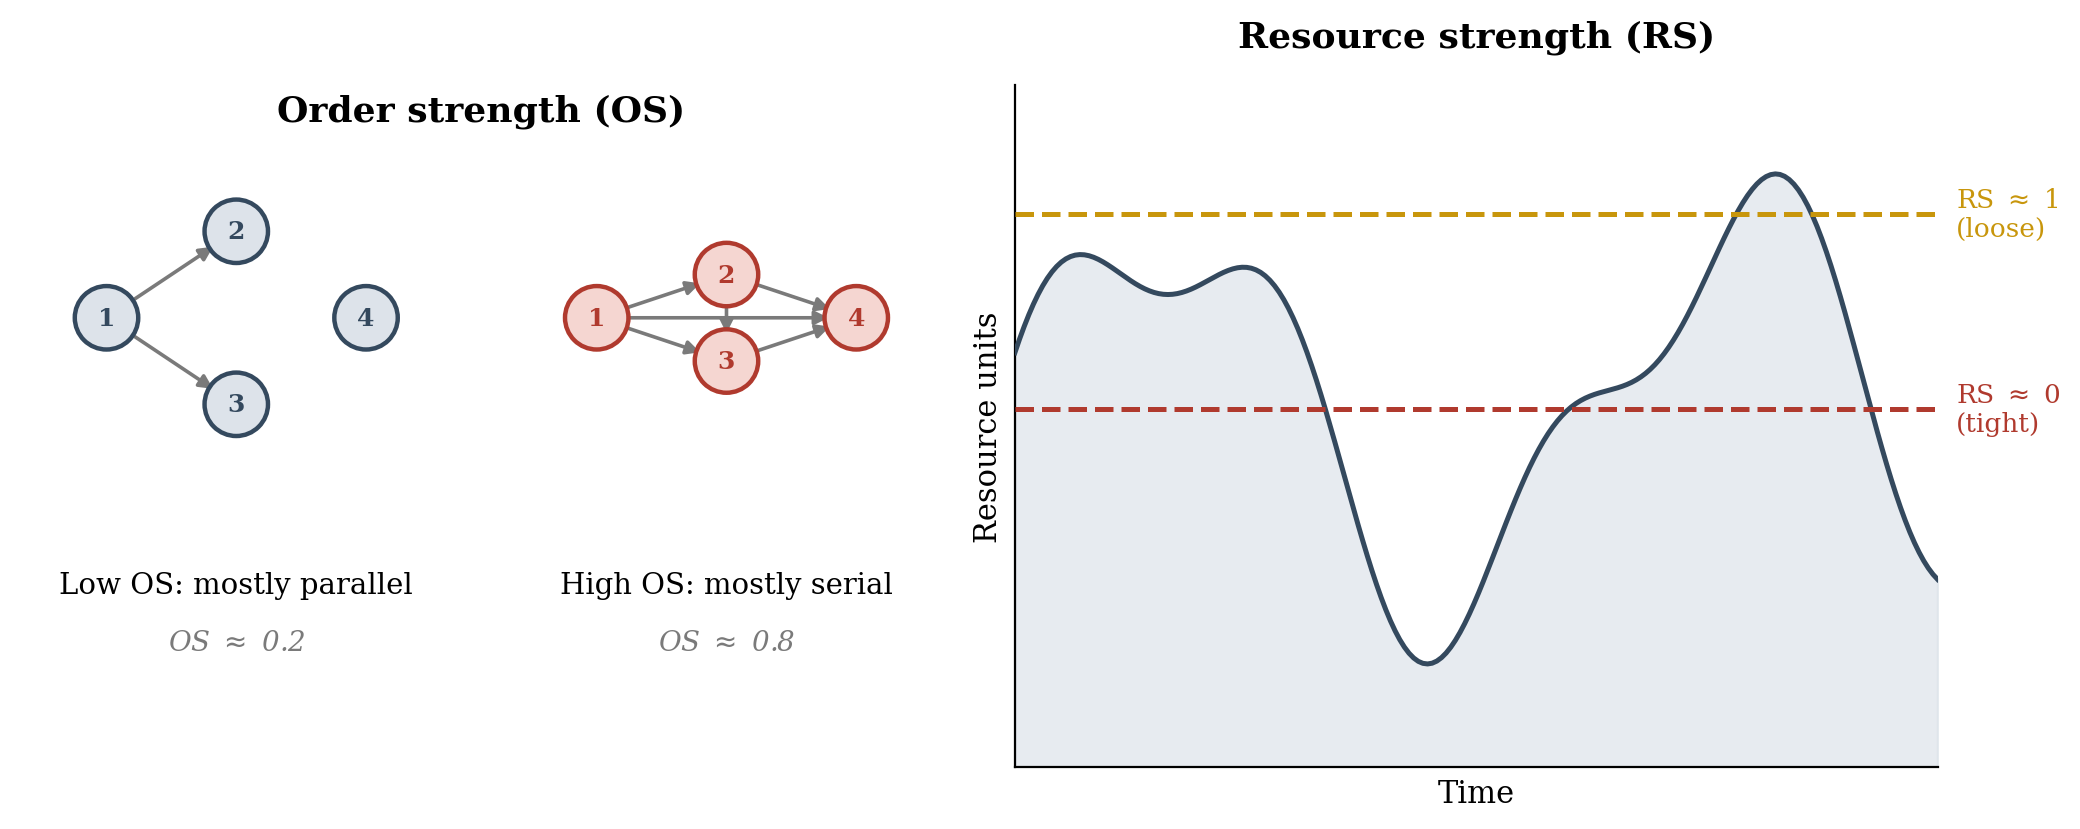
\includegraphics[width=0.95\textwidth]{img/instance-indicators.png}
  \caption[Order strength and resource strength, illustrated]{Order strength
  (OS) and resource strength (RS) illustrated on small synthetic examples.
  Left: a low-OS precedence graph (many parallel activities) versus a
  high-OS graph (a near-serial chain). Right: \changed{the solid curve is
  the aggregate demand for one renewable resource over time under an
  earliest-start schedule; the two dashed horizontal lines are two
  alternative per-period availability levels for the same demand profile.
  An availability well above the demand peak gives a loose instance
  ($\mathrm{RS}\approx 1$), an availability close to the unavoidable
  minimum a tight one ($\mathrm{RS}\approx 0$).} Resource factor (RF) is
  omitted as it is a simple counting indicator with no useful graphical
  analogue.}
  \label{fig:instance-indicators}
\end{figure}

%==============================================================================
\section{Schedule quality evaluation metrics}
\label{sec:eval-metrics}
%==============================================================================

A \emph{schedule} for an MRCPSP instance assigns every activity a mode
$m \in \mathcal{M}_i$ and a start time, and is \emph{feasible} if it satisfies the
three constraint classes of Section~\ref{subsec:problem-statement}:
precedence, per-period renewable-resource availability, and total
nonrenewable-resource budgets. Only feasible schedules are considered; the
schedule-generation scheme used throughout this thesis (and by the baseline)
constructs feasible schedules by design, so feasibility itself is not used as
a ranking criterion; schedules are compared purely on quality.

The primary quality measure is the \emph{makespan} $C_{\max}$, the completion
time of the sink activity, as already defined in
Section~\ref{subsec:cpm}. Because $C_{\max}$ depends strongly on instance
size, it cannot be compared directly across instances of different $n$, OS,
RF or RS. Following standard practice in the (M)RCPSP
literature~\cite{kolisch1997,vanpeteghem2014}, $C_{\max}$ is therefore
normalised against an instance-specific lower bound before being aggregated.

\textbf{CPM-based lower bound.} For instance $i$, let
$d_{i}^{\min} = \min_{m \in \mathcal{M}_i} d_{im}$ be the duration of its shortest
mode. Applying the forward CPM recursion of
Section~\ref{subsec:passes}, equations~\eqref{eq:es}--\eqref{eq:ef}, with
$d_{i}^{\min}$ in place of $d_i$ and \emph{ignoring all resource
constraints} gives the earliest finish (EF) time of the sink activity, denoted
$\mathrm{CPM}_{\mathrm{EF}}(i)$. Since both the resource constraints and the
choice of (possibly longer) modes are relaxed, $\mathrm{CPM}_{\mathrm{EF}}(i)$
is a valid, though generally not tight, lower bound on $C_{\max}(i)$ for
any feasible schedule of instance $i$, and depends only on the instance, not
on the algorithm being evaluated.

\textbf{Relative deviation.} The quality of a schedule with makespan
$C_{\max}(i)$ on instance $i$ is reported as its percentage deviation from
this lower bound,
\[
  \mathrm{dev}(i) \;=\; \frac{C_{\max}(i) - \mathrm{CPM}_{\mathrm{EF}}(i)}{\mathrm{CPM}_{\mathrm{EF}}(i)} \times 100\%.
\]
Averaging $\mathrm{dev}(i)$ over a set of instances (training, validation or
test) gives the \emph{Average Relative Deviation} (ARD\%), the single number
used both as the GP fitness function during training
(Section~\ref{subsec:problem-statement}, Chapter~\ref{chap:approach}) and as
the headline figure for comparing configurations and reporting results in
Chapter~\ref{chap:experiments}.

\textbf{Statistical comparison.} Because $\mathrm{dev}(i)$ is computed for
every algorithm configuration on the same instances, two configurations can
be compared instance-by-instance using a paired, non-parametric Wilcoxon
signed-rank test on the per-instance deviations. Chapter~\ref{chap:experiments}
reports such comparisons against the baseline using a one-sided test (the
alternative hypothesis being that the proposed configuration's deviations are
\emph{lower}), marking improvements as significant at the $p<0.05$ and
$p<0.10$ levels.
